%!TEX root = ../main.tex

\chapter{基于有效字符的Web内容抽取}

\section{概述}
在Internet时代,Web新闻和博客都是很有代表性的信息发布和获取渠道。

Web新闻区别于传统的报纸,在互联网上发布意味着它能够触及更广大的受众,扩大自己的影响力,
对热点新闻的实时推送也提高了信息传播的即时性。
阅读Web新闻了解实事动态已经成为广大网民的生活习惯,很多传统媒体也纷纷推出了自己的Web新闻。

博客(blog,weblog的缩写,也叫网络日志)是发布在互联网上的文章集合,通常由个人撰写和管理。
博客给普通大众提供了一个表达自己观点和态度的平台,人们还能在文章后发表评论,
形成一个庞大的社区,促进信息的交流。

但除了新闻正文之外,一个典型的新闻网页还包含导航栏、广告、推荐链接和版权信息等,
这些与正文无关的额外内容,通常称为噪声。
Gibson在2005年的研究\cite{gibson2005volume}显示,
网页模板在整个网页中占据了$40\%$--$50\%$的字节量,而且这个比例正以每年$6\%$的速度增长。
以一篇新浪新闻\footnote{http://news.sina.com.cn}为例,如图~\ref{fig:news}~所示,
红色实线圈出的内容都与正文无关,它们占据了网页一半以上的篇幅。

博客和新闻类似,都属于正文集中的网站,博客网页的噪声主要有导航栏、广告和博客相关文章等。
以一篇网易博客\footnote{http://blog.163.com}为例,如图~\ref{fig:blog}~所示,
红色实线圈出的是与正文无关的内容。

\begin{figure}[htbp]
\centering
\includegraphics[width=0.9\textwidth,height=0.45\textheight]{news}
\caption{新浪新闻实例}
\label{fig:news}
\end{figure}

\begin{figure}[htbp]
\centering

\includegraphics[width=0.9\textwidth,height=0.45\textheight]{blog}
\caption{网易博客实例}
\label{fig:blog}
\end{figure}

从网页中抽取核心内容,过滤这些噪声,不仅能够给用户提供“干净”的内容,
也能节约爬虫系统的存储开销,减小索引规模,提升后续自然语言处理的效果。
由于新闻和博客网页布局与内容抽取目标的相似性,本章将两者合并处理,
提出一种基于有效字符的Web内容抽取方法,~\ref{sec:cevc-method}~节详述该方法CEVC,
~\ref{sec:cevc-alternative}~节简述对比方法CETR和CETD,
~\ref{sec:cevc-experiment}~节进行对比实验并分析结果。

\section{CEVC方法}
\label{sec:cevc-method}

\subsection{DOM}
DOM(Document Object Model,文档对象模型)是一个跨平台语言无关的规范,
用来表示和操作HTML,XHTML和XML的对象\footnote{http://www.w3.org/DOM/}。
每个文档所包含的节点被组织为一个树型结构,称为DOM树。
DOM树节点所表示的对象可以通过一组方法来寻址或操作,这些接口以API的形式描述。
通过这样一种规范,程序和脚本能够动态访问和更新文档的内容、结构以及风格,
文档经过后续处理后,还能将结果更新到展示的页面上。

上世纪90年代,网景公司和微软公司相继推出自己的浏览器,和浏览器端的脚本语言JavaScript。
JavaScript让Web开发者能够创造和用户交互的网页,检测用户产生的事件并更新HTML文档,
这类第一代的语言被称为Legacy DOM。
随后W3C(World Wide Web Consortium,万维网联盟)制定了第一版的DOM标准,
之后相继发布了新版本。
截止到2005年,W3C DOM中的大部分特性都能被主流浏览器广泛支持。

HTML文档可以解析为DOM树,每个HTML标签对应一个DOM树节点,
父子节点对应HTML标签的嵌套关系,兄弟节点对应HTML标签的并列关系,
这样就把序列化的HTML文档转换为层次化的对象模型,便于程序的访问和操作。

\begin{figure}[htbp]
\begin{example}
\label{ex:html}
一个简化的HTML代码片段
\end{example}
\begin{verbatim}
 1. <html>
 2.   <head> ... </head>
 3.   <body>
 4.     <div class="nav-wrap">
 5.       <h1>News Title</h1>
 6.     </div>
 7.     <div> ... </div>
 8.     <div class="ep-content">
 9.       <a>
10.         <span>From WWW</span>
11.       </a>
12.       <p>First paragraph.</p>
13.       <p>Second paragraph.</p>
14.     </div>
15.   </body>
16. </html>
\end{verbatim}
\end{figure}

\begin{figure}[htbp]
\centering
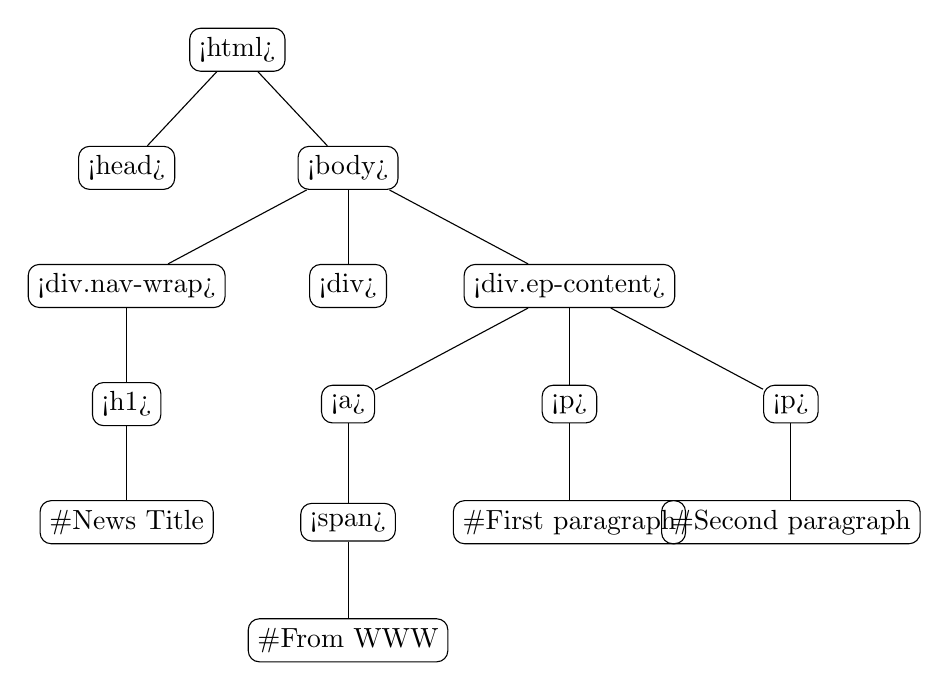
\begin{tikzpicture}[
sibling distance=8em,
every node/.style={rectangle,rounded corners,draw},
]
\node{<html>}
  child{node{<head>}}
  child{node{<body>}
    child{node{<div.nav-wrap>}
      child{node{<h1>}
        child{node{\#News Title}}
      }
    }
    child{node{<div>}}
    child{node{<div.ep-content>}
      child{node{<a>}
        child{node{<span>}
          child{node{\#From WWW}}
        }
      }
      child{node{<p>}
        child{node{\#First paragraph}}
      }
      child{node{<p>}
        child{node{\#Second paragraph}}
      }
    }
  }
;
\end{tikzpicture}
\caption{一个简化的DOM树}
\label{fig:dom}
\end{figure}

例~\ref{ex:html}~所示的HTML片段经过解析后形成一个DOM树,如图~\ref{fig:dom}~所示。
每个HTML标签都与一个DOM树节点对应,HTML标签的属性仍然附属在DOM节点上。
网页中能够显示的具体文本都位于DOM树的叶节点上,DOM树的内部节点只负责结构控制和布局。
HTML的根节点是\texttt{<html>},一般包含两个节点\texttt{<head>}和\texttt{<body>}。
网页的可视区域都从\texttt{<body>}标签开始,
因此我们的研究对象是\texttt{<body>}标签下的内容。

\subsection{有效字符}
回顾图~\ref{fig:news}~和~\ref{fig:blog}~,我们注意到网页正文一般是文本密集的区域,
而噪声信息则包含高度格式化的、简短的文本。
通过大量实例分析,我们发现噪声信息通常包含链接,无论是导航栏的网站板块链接,
还是广告链接或相关文章链接,它们都符合这个特点,吸引用户点击来完成自己的职能。
反之,一段不包含链接的文本更有可能是网页核心内容。

链接在HTML文档中由\texttt{<a>}标签组成,a代表anchor,所以链接内的文本也称为锚文本。
DOM节点的继承关系使得包裹在\texttt{<a>}标签内的所有文本都变成锚文本,
例如图~\ref{fig:dom}~中的\texttt{From WWW}虽然在\texttt{<span>}下,
但其祖先节点是一个\texttt{<a>}标签,因此也变成了锚文本。

除此之外,噪声信息较为简短,甚至不能组成一个语义完整的句子,我们可以利用停止词来刻画这一特征。
停止词是自然语言处理中过滤掉的词\footnote{https://en.wikipedia.org/wiki/Stop\_words},
它们在一篇文章中大量出现,多为冠词、介词或连词,却对文章主体内容贡献很小。
尽管停止词对文章没有多大意义,但一段话如果没有停止词,那么它就不是一个语义完整的句子,
更有可能是一组关键词的堆砌,而不是网页的核心内容。
例~\ref{ex:stopwords}~节选自网页中的一段话,以\texttt{<>}的形式标注了其中的停止词,
可见停止词在正文中是普遍存在的。

\begin{figure}[htbp]
\begin{example}
\label{ex:stopwords}
网页中的停止词示例
\end{example}
买房<还是>租房?<这是>眼下很多<人>要面对<的>一道选择题。
如果简单比较,一边<是>数额很大<的>买房负担,
一边<是>相对<可>接受<的>租金价格,似乎租房应更受欢迎,现实<却>非如此。
山东某县一位购房者对笔者道出心声:“买房子,政府一平方米补贴100元,一套房子能省1万多元。
租房子,<啥>实惠没有,<还>总<被>赶来赶去,住<着不>踏实。”
<他>最终<还是>选择<了>勒紧裤腰带贷款买房。
\end{figure}

结合上述链接和停止词与网页噪声的相关性,我们提出一个有效字符的概念:

\begin{definition}
\label{def:validchar}
$i$是DOM中的一个叶节点,如果$\forall p \in ancestors(i)$都有$tag(p) \neq a$,
并且$stopwords(i) > 0$,那么$i$所包含的文本就是有效字符。
\end{definition}

定义~\ref{def:validchar}~中,$ancestors(i)$表示$i$的所有祖先节点,
$tag(p)$表示$p$的标签名,$stopwords(i)$表示$i$的停止词个数。
有效字符代表网页中那些更有可能是正文的文本,忽略了链接噪声和太过松散的短语,
有效字符越多,代表这个节点更有可能是正文。

为了利用DOM节点的有效字符分布信息,我们需要计算每个DOM节点下所包含的有效字符个数,
可以将其作为一项属性,插入到DOM节点中,便于后续的处理。
在计算之前,首先去除网页中的\texttt{<script>},\texttt{<style>}和\texttt{comment}。
这些脚本、样式文件和注释对网页显示的文本内容没有贡献,却可能干扰计算结果。

如算法~\ref{algo:cevc-count}~所示,这是一个自顶向下的递归计算过程。
ValidChars被作为属性,存储在节点中。
当前节点有子节点时,递归计算子节点,然后当前节点的有效字符数被累加到父节点上。
当前节点是叶节点时,根据定义~\ref{def:validchar}~判断它包含的文本是否是有效字符,
如果是,则将非空白字符数累加到父节点上。
这里忽略了空白字符,是为了排除网页排版风格带来的影响,让计算结果更加稳定。

算法~\ref{algo:cevc-count}~的主要操作就是遍历DOM树,
所以它的运行时间与DOM树中的节点数成正比,时间复杂度为$O(n)$,$n$是DOM树中的节点数。
为了在内存中存储解析后的DOM树,其空间复杂度也是$O(n)$。

\begin{algorithm}[htbp]
\caption{countValidChars(N)}
\label{algo:cevc-count}
\KwIn{DOM node N}
\KwOut{DOM node N}

\eIf{N has child nodes} {
  \For{C $\in$ N.children()}{
    countValidChars(C) \;
  }
  N.parent.validChars += N.validChars \;
}{
  \tcp{N is a leaf text node}
  \If{N consists of valid characters}{
    length = getNonSpaceLength(N) \;
    N.parent.validChars += length \;
  }
}
\end{algorithm}

经过算法~\ref{algo:cevc-count}~的处理,
我们可以得到一个标注了各个节点ValidChars的HTML页面,如图~\ref{fig:validchar}~所示。

\begin{figure}[t]
\centering
\includegraphics[width=0.9\textwidth]{figures/新闻划分}
\caption{有效字符示例}
\label{fig:validchar}
\end{figure}

\subsection{定位核心内容块}
经过大量实例分析,我们发现对于新闻、博客这类正文信息集中的网站,
核心内容块都位于同一个父节点之下,通常表现为文本的段落。
图~\ref{fig:validchar}~中的新闻正文位于\texttt{<div\#endText>}节点之下,
是由\texttt{<p>}标签构成的段落。

现在我们看到每个DOM节点上都标注了有效字符的个数,有效字符越多表明这个节点越可能是核心内容。
但这个比较必须在同一个层次的兄弟节点间才有意义,因为有效字符数是嵌套包含的,
毫无疑问\texttt{<body>}的有效字符数最多。
如果从\texttt{<body>}节点开始,每次都选择有效字符数最多的子节点深入,
就能定位出一条从\texttt{<body>}通往核心内容块的正确路径,
如图~\ref{fig:validchar}~中红线标示的节点。

每次沿着有效字符数最大的子节点不断深入,意味着我们每一步放弃了信息量较小的兄弟节点。
这个过程不能一直持续下去,否则会陷入到叶节点中,而错失最终的父节点。
如图~\ref{fig:validchar}~所示,最后一步进入了一个\texttt{<p>}标签,
而错失了真正的核心内容块\texttt{<div\#endText>}。
我们需要定义一个指标,来判断何时停止向下深入的过程。

\begin{definition}
\label{def:mcr}
$i$是DOM树中的一个节点,$i$的最大子节点字符占比MCR(Max Chars Ratio)如下所示,
其中$C_i$表示$i$的有效字符数,$j$是$i$的子节点:
\begin{equation}
MCR_i = max_{j \in children(i)} \frac{C_j}{C_i}
\end{equation}
\end{definition}

在DOM树中每次向下深入一步,我们认为最大子节点包含了父节点的绝大部分文本信息。
当定义~\ref{def:mcr}~中的MCR低于一个阈值时,
表明最大子节点的有效字符数并不足以在父节点中占据统治地位,
即最大子节点的文本不能在可接受的损失范围内代表父节点,这时候放弃兄弟节点是不合理的,
因此向下深入的过程应立即终止,当前节点就是核心内容块。

\begin{figure}[htbp]
\begin{example}
\label{ex:mcr}
MCR计算过程
\end{example}
\begin{verbatim}
1. <body> valid_chars=4161 MCR=0.99
2. <div#js-epContent> valid_chars=4102 MCR=1.0
3. <div.ep-content-bg> valid_chars=4102 MCR=0.95
4. <div#epContentLeft> valid_chars=3912 MCR=0.94
5. <div#endText> valid_chars=3685 MCR=0.14 核心内容块
6. <p> valid_chars=505
\end{verbatim}
\end{figure}

如例~\ref{ex:mcr}~所示,每一行显示的都是图~\ref{fig:validchar}~中各层的最大子节点。
在到达\texttt{<body\#endText>}之前,MCR一直保持$0.9$以上的高比率,
而\texttt{<body\#endText>}的MCR锐减到$0.14$,因为此时已深入到正文的一个段落中,
这个段落无法代表正文的内容,\texttt{<body\#endText>}就是最终的核心内容块。

上述过程如算法~\ref{algo:cevc-stepinto}~所示。
在经过算法~\ref{algo:cevc-stepinto}~\texttt{countValidChars}预处理后的DOM树上,
先遍历子节点,找出有效字符数最大的子节点,并累加所有字符数。
然后选定最大子节点\texttt{maxNode},如果MCR小于一个阈值$\alpha$就停止并输出当前节点,
否则在MaxNode上继续递归调用算法\texttt{stepInto}。
\texttt{output}过程负责把当前节点的所有有效字符输出,作为核心内容抽取的结果返回。
注意第~\ref{algo:line:edge}~行,当遇到一种极端情况,正文仅仅包含一个段落,
那么StepInto深入到最底层仍然会有很高的MCR,导致无法终止直到进入叶节点。
这时候采取一种简单的策略,认为当前节点的父节点就是核心内容块。
后续实验表明,这是一个简单也可以接受的方案。

算法~\ref{algo:cevc-stepinto}~能够很快运行结束,因为它至多被递归调用$h$次,
$h$是DOM树的深度,时间复杂度为$O(h)$。

\begin{algorithm}[htbp]
\caption{stepInto(N)}
\label{algo:cevc-stepinto}
\KwIn{DOM node N}
\KwOut{main content}

maxNode = null \;
maxValidChars = 0 \;
totalValidChars = 0 \;
\For{$C \in N.children()$}{
  totalValidChars += C.validChars \;
  \If{$C.validChars > maxValidChars$}{
    maxValidChars = C.validChars \;
    maxNode = C \;
  }
}

\eIf{maxNode is not null}{
  MCR = maxValidChars / totalValidChars \;
  \eIf{$MCR < \alpha$}{
    \Return output(N) \;
  }{
    stepInto(maxNode) \;
  }
}{
  \tcp{Step into the leaf node}
  \Return output(N.parent) \; \label{algo:line:edge}
}
\end{algorithm}

\section{对比方法}
\label{sec:cevc-alternative}

\section{实验与分析}
\label{sec:cevc-experiment}
